\documentclass[12pt,a4paper]{article}

% ===== Codificação / fontes (XeLaTeX) =====
\usepackage{fontspec}
\usepackage{polyglossia}
\setmainlanguage{portuguese}
\setmainfont{Latin Modern Roman}

% ===== Pacotes =====
\usepackage{amsmath,amssymb}
\usepackage{geometry}
\geometry{margin=2.5cm}
\usepackage{graphicx}
\graphicspath{{../outputs/figuras/}}
\usepackage{booktabs}
\usepackage{caption}
\usepackage{subcaption}
\usepackage{float}
\usepackage[hidelinks]{hyperref}
\usepackage{natbib}
\bibliographystyle{apalike}
\usepackage{setspace}
\onehalfspacing
\usepackage{siunitx}
\sisetup{group-separator={.},group-minimum-digits=4,output-decimal-marker={,}}
\usepackage[protrusion=true]{microtype}
\emergencystretch=3em  % absorve estouros residuais de margem em prosa justificada

\title{\textbf{A reforma do seguro-desemprego de 2015 é identificável em séries agregadas?}\\[4pt]
\large Uma avaliação por séries temporais interrompidas e os limites da identificação macroeconômica}

\author{Arthur Donato\\
\small PPGE --- FURG (Mestrado em Economia Aplicada)}

\date{\today}

\begin{document}
\maketitle

\begin{abstract}
\noindent A Lei n\textsuperscript{o}~13.134/2015 endureceu o acesso ao seguro-desemprego (SD) no Brasil, elevando de 6 para 12 meses o tempo mínimo de vínculo exigido na primeira solicitação. Avaliamos o efeito dessa reforma sobre o número mensal de requerentes do SD (2000--2025, 304 meses) por triangulação de dois métodos de série temporal interrompida (ITS): ARIMA de intervenção com contrafactual e o modelo estrutural bayesiano \textit{CausalImpact} (BSTS). Em nível, os dois métodos convergem em uma queda de aproximadamente \textbf{16\%} ($\approx$114 mil requerentes/mês) após julho de 2015. Esse resultado, porém, \textbf{não sobrevive} à inclusão das demissões do CAGED como covariável de controle: o efeito desaparece ($+2{,}6\%$, $p\approx0{,}15$) e o intervalo de credibilidade encolhe pela metade. Especificações alternativas sobre a taxa de habilitação (requerentes/demissões) divergem em sinal. A conclusão central é metodológica: o efeito da reforma \textbf{não é robustamente identificável com dados agregados nacionais}, porque a Lei coincidiu com a recessão de 2015--16, que moveu simultaneamente o volume de demissões, a composição das separações e o \textit{take-up}. O estudo delimita, assim, a fronteira de identificação do problema e motiva um desenho de descontinuidade de elegibilidade (RD/DiD) em microdados.

\medskip
\noindent\textbf{Palavras-chave:} seguro-desemprego; Lei 13.134/2015; séries temporais interrompidas; CausalImpact; identificação causal.\\
\textbf{Classificação JEL:} J65, C22, H55.
\end{abstract}

% =====================================================================
\section{Introdução}
% =====================================================================

O seguro-desemprego (SD) é o principal instrumento de proteção de renda ao trabalhador formal demitido no Brasil. Como todo programa de seguro social, ele carrega um \textit{trade-off} central: provê liquidez e suavização de consumo a quem perde o emprego, mas pode distorcer a intensidade da busca por recolocação \citep{baily1978optimal,chetty2008moral}. Em economias com amplo setor informal, esse cálculo de bem-estar é modificado pela possibilidade de transição para a informalidade \citep{gerardgonzaga2021informal}.

Em dezembro de 2014 o Governo Federal editou a MP~665, convertida na \textbf{Lei n\textsuperscript{o}~13.134, de 16 de junho de 2015} \citep{lei13134_2015}, que endureceu o acesso ao benefício. A mudança mais saliente foi o tempo mínimo de vínculo exigido para a \textbf{primeira solicitação}, que subiu de cerca de 6 para \textbf{12 meses} nos últimos 18 (a segunda solicitação passou a exigir 9 meses; a terceira em diante permaneceu em 6). O governo projetava economia da ordem de R\$~6,4 bilhões e cerca de 1,6 milhão de trabalhadores (19\%) fora do benefício já em 2015.

Apesar da relevância fiscal e social da reforma, \textbf{avaliações causais dedicadas são escassas}. A referência mais próxima é descritiva \citep{amorim2024perfil}, baseada em tabulações anuais da Base de Gestão do Seguro-Desemprego (BGSD). Este trabalho parte dessa lacuna e pergunta: \textit{qual foi o efeito da Lei 13.134/2015 sobre o fluxo de requerentes do SD?} Mais importante, documenta \textit{se} essa pergunta pode ser respondida com os dados agregados disponíveis.

A contribuição é dupla. Primeiro, oferecemos a primeira avaliação quantitativa da reforma de 2015 com a série mensal completa (2000--2025) por triangulação de dois métodos de série temporal interrompida. Segundo --- e este é o achado central --- mostramos que o efeito aparente de $-16\%$ em nível é \textbf{confundido pela recessão de 2015--16}: ao controlar pela dinâmica de demissões, o efeito desaparece, e especificações concorrentes divergem em sinal. O resultado é, portanto, uma \emph{nota de não-identificação}: delimitamos o que os dados agregados conseguem e o que não conseguem sustentar, e derivamos daí o desenho de microdados necessário para uma identificação limpa.

% =====================================================================
\section{Revisão de literatura}
% =====================================================================

\subsection{Teoria: seguro versus incentivo}
O arcabouço moderno do SD ótimo origina-se em \citet{baily1978optimal}, que formaliza o \textit{trade-off} entre suavização de consumo e distorção da busca. \citet{chetty2008moral} reformula o problema decompondo o efeito do benefício sobre a duração do desemprego em uma parcela de \textbf{liquidez} (desejável, corrige mercados de crédito incompletos) e uma parcela de \textbf{moral hazard} (distorção de incentivo); estima que cerca de 60\% do efeito é liquidez, o que justifica benefícios relativamente generosos. \citet{cardchettyweber2007cash} fornecem a evidência de que o \textit{cash-on-hand} afeta a duração da busca, sustentando o canal de liquidez.

\subsection{Evidência quase-experimental internacional}
A fronteira empírica é quase-experimental. \citet{schmiedervonwachter2016effects} sintetizam duas décadas de estimativas (sobretudo RD na Alemanha) e concluem que os efeitos de nível e duração do benefício são pequenos a modestos, com efeito aproximadamente nulo sobre a qualidade média do emprego; extensões em recessão não elevam a duração de forma duradoura. \citet{nekoeiweber2017does}, por sua vez, encontram que estender o SD pode \textit{melhorar} a qualidade do reemprego (melhor \textit{match}). Os padrões de \textit{hazard} de saída e os \textit{spikes} na exaustão do benefício foram estabelecidos por \citet{katzmeyer1990impact} e \citet{meyer1990unemployment}; \citet{lalive2008how} é um template clássico de RD sobre regras de duração.

\subsection{Seguro-desemprego no Brasil}
A agenda brasileira foi transformada pelos microdados administrativos ligados (RAIS/CAGED/registro do SD). O tema dominante é a \textbf{margem informal}: \citet{gerardgonzaga2021informal} mostram que o custo de eficiência do SD é \textit{menor} em mercados mais informais; \citet{britto2022employment} compara proteção \textit{lump-sum} (FGTS/multa) e contingente (SD), concluindo que o SD induz transição para a informalidade mas ainda assim é preferível; \citet{brittopinottisampaio2022crime} usam RD na elegibilidade e mostram que o SD anula o aumento de criminalidade pós-demissão enquanto o benefício dura. Esse último desenho --- \textbf{RD na descontinuidade de elegibilidade} --- é diretamente transponível para a reforma de 2015. No plano descritivo, \citet{amorim2024perfil} perfilam o acesso repetido ao SD na BGSD e documentam a redução de beneficiários após 2015; \citet{balbinottozylberstajn2002uso} e \citet{gonzaga2003labor} fornecem o pano de fundo histórico (reincidência e rotatividade elevada).

\subsection{Métodos de avaliação em séries agregadas}
Quando o desenho de microdados não está disponível, a avaliação recorre a séries temporais interrompidas (ITS). O modelo ARIMA de intervenção remonta a \citet{boxtiao1975intervention}; o tutorial de \citet{bernal2017interrupted} sistematiza o uso de ITS em avaliação de políticas; a implementação automática de seleção de ordem está em \citet{hyndmankhandakar2008forecast}. O \textit{CausalImpact} \citep{brodersen2015causalimpact} generaliza a ITS para um modelo estrutural bayesiano de séries temporais (BSTS) com contrafactual, acomodando covariáveis de controle. A lacuna que todos esses métodos agregados enfrentam --- e que este artigo torna explícita --- é o confundidor macroeconômico contemporâneo à intervenção; a saída reconhecida pela literatura brasileira é a RD na elegibilidade \citep{leelemieux2010rdd,calonico2014robust,brittopinottisampaio2022crime} e o DiD com múltiplos períodos \citep{callawaysantanna2021did}.

% =====================================================================
\section{Dados}
% =====================================================================

A variável de interesse é o \textbf{número mensal de requerentes do seguro-desemprego} (trabalhador formal, Brasil), extraído da \textit{Série Histórica do Seguro-Desemprego} da Base de Gestão do Seguro-Desemprego (BGSD), MTE/SPPE. A cobertura é \textbf{mensal, de janeiro de 2000 a abril de 2025} (304 observações), por UF de demissão e para o agregado nacional. A série é contínua, sem lacunas ou valores ausentes.

A escolha da série mensal é deliberada. O estudo descritivo que motivou o projeto \citep{amorim2024perfil} usa apenas o agregado \textit{anual} até 2019, insuficiente para modelagem de série temporal --- o que torna a série mensal completa (até 2025) a "necessidade de completar a série".

Como \textbf{controle} para a dinâmica do mercado de trabalho na especificação do \textit{CausalImpact}, usamos as admissões e demissões mensais do \textbf{CAGED antigo} (séries \texttt{CAGED12\_ADMIS} e \texttt{CAGED12\_DESLIG}, IPEADATA/MTE, 1999-05 a 2019-12). O controle só se aplica à janela da Lei de 2015 (toda pré-2020, antes da quebra do Novo CAGED). A correlação pré-intervenção entre demissões e requerentes é de \textbf{0,93}, o que torna as demissões um preditor forte do contrafactual.

A Figura~\ref{fig:serie} apresenta a série de requerentes com as duas intervenções datadas, e a Figura~\ref{fig:stl} sua decomposição STL (tendência, sazonalidade, resíduo).

\begin{figure}[H]
\centering
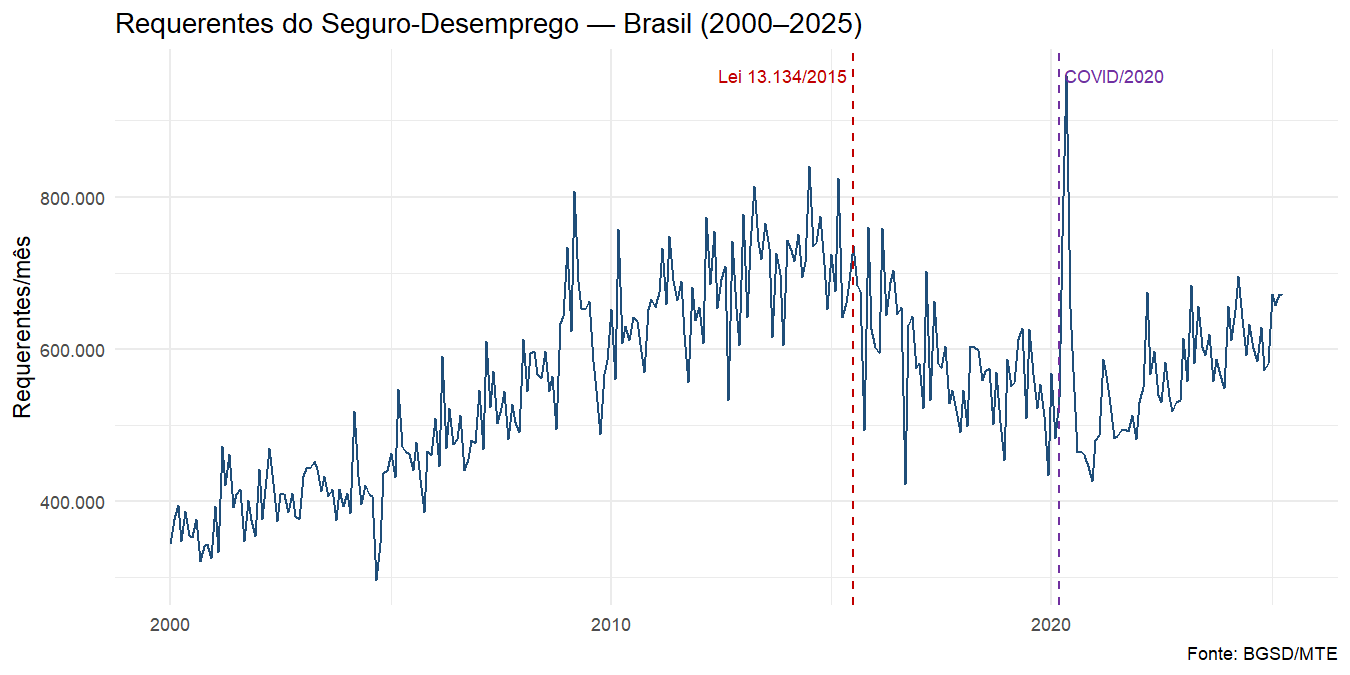
\includegraphics[width=0.92\textwidth]{01_serie_requerentes.png}
\caption{Requerentes mensais do seguro-desemprego (Brasil, 2000--2025), com as intervenções avaliadas: Lei 13.134/2015 (jul/2015) e choque pandêmico (mar/2020).}
\label{fig:serie}
\end{figure}

\begin{figure}[H]
\centering
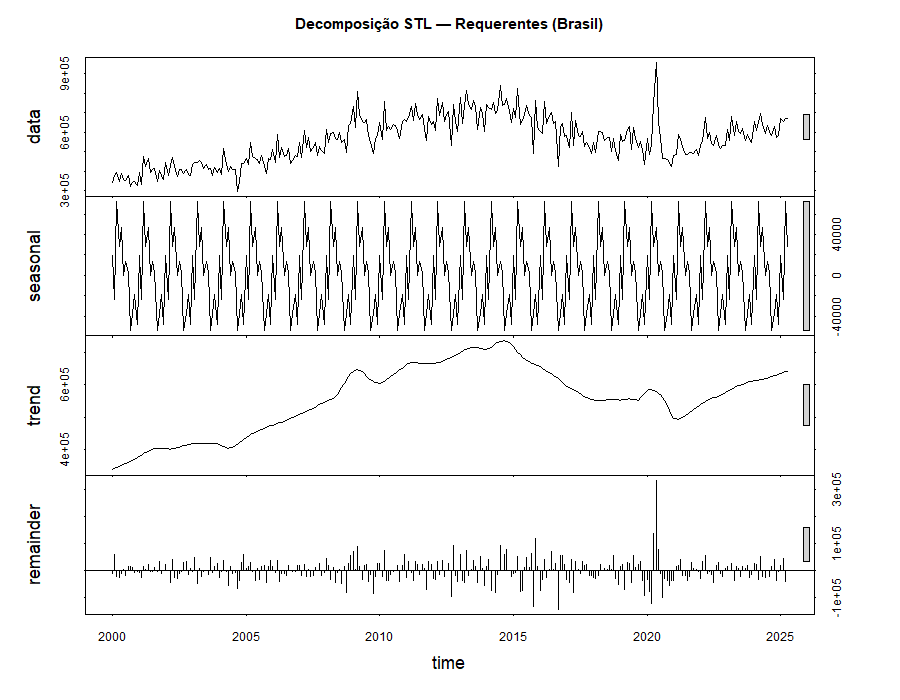
\includegraphics[width=0.92\textwidth]{02_stl_decomposicao.png}
\caption{Decomposição STL da série de requerentes: tendência de longo prazo, sazonalidade mensal e componente remanescente.}
\label{fig:stl}
\end{figure}

% =====================================================================
\section{Metodologia}
% =====================================================================

Avaliamos duas intervenções: a \textbf{Lei 13.134/2015} (jul/2015), esperada como um degrau permanente de queda, e o \textbf{choque pandêmico} (mar/2020), esperado como pulso agudo seguido de vale. A estratégia é de \textbf{triangulação}: dois métodos ITS independentes, com janelas idênticas, cujas concordâncias e discordâncias são informativas.

\subsection{ARIMA de intervenção (contrafactual)}
A série de requerentes é não estacionária em nível: o teste ADF não rejeita a raiz unitária ($p = 0{,}27$) e o KPSS rejeita a estacionariedade ($p < 0{,}01$); os critérios automáticos sugerem uma diferença regular ($d=1$) e nenhuma sazonal ($D=0$). Ajustamos um modelo SARIMA \textbf{apenas na janela pré-intervenção} e projetamos o contrafactual para o período pós-intervenção. O efeito é a diferença entre o observado e o contrafactual previsto,
\[
\widehat{\tau}_t = y_t - \widehat{y}_t^{\,\text{contraf}}, \qquad t > T_0,
\]
com intervalos derivados da distribuição preditiva. Para a Lei de 2015 o modelo selecionado foi um ARIMA(0,1,4)(1,0,0)[12] (186 meses de pré-período); para o COVID, um ARIMA(3,1,1)(1,0,0)[12]. Como robustez, estimamos também um modelo Box--Tiao com \textit{dummies} de intervenção \citep{boxtiao1975intervention}; ressalve-se que, sob $d=1$, o termo de \textbf{degrau} é mal identificado, ao passo que o \textbf{pulso} (COVID) é estimado com confiança.

\subsection{CausalImpact (BSTS)}
O segundo método é o modelo estrutural bayesiano de séries temporais de \citet{brodersen2015causalimpact}, com componente de tendência local e sazonalidade mensal. Na especificação \textbf{sem controle}, o contrafactual é projetado a partir da própria dinâmica pré-intervenção. Na especificação \textbf{com controle}, incluímos as demissões do CAGED como série preditora, de modo que o contrafactual passa a condicionar na trajetória contemporânea do mercado de trabalho. A comparação entre as duas é o teste decisivo do artigo: se o efeito de $-16\%$ é um artefato da recessão, ele deve atenuar-se ao controlar pelas demissões.

\subsection{Teste da taxa de habilitação}
Como verificação adicional, modelamos a \textbf{taxa de habilitação} --- a razão requerentes/demissões (e segurados/demissões). O raciocínio: se a Lei operou endurecendo a elegibilidade, essa razão deveria \textit{cair} após 2015, independentemente do volume de demissões. Confrontamos quatro estimativas agregadas (nível sem controle; condicional a demissões; taxa contra contrafactual; médias simples pré$\to$pós) para avaliar a robustez do sinal.

\paragraph{Ressalva do denominador.} O denominador utilizado é o \textit{total} de desligamentos; o correto seria restringir à \textbf{dispensa sem justa causa}, categoria que efetivamente aciona o SD. Como a recessão eleva a fração de separações involuntárias, parte de qualquer movimento na taxa reflete \textbf{composição}, não a Lei. O código de layout do CAGED antigo (código 31) permite construir esse denominador correto, pendente apenas do acesso aos microdados.

% =====================================================================
\section{Resultados}
% =====================================================================

\subsection{Efeito bruto: os dois métodos convergem em $-16\%$}
Em nível, ARIMA-ITS e CausalImpact concordam de forma marcante (Tabela~\ref{tab:triang}). Para a Lei de 2015, o ARIMA-ITS estima $-$\num{113056} requerentes/mês ($-16{,}2\%$; IC 95\% $[-$\num{276750}$, +$\num{50638}$]$) e o CausalImpact estima $-$\num{115142} requerentes/mês ($-16{,}4\%$; IC 95\% $[-$\num{173436}$, -$\num{59941}]$, $p\approx0{,}001$). As figuras de ajuste constam das Figuras~\ref{fig:its2015}--\ref{fig:ci2015}.

\begin{table}[H]
\centering
\caption{Triangulação dos efeitos médios sobre requerentes/mês.}
\label{tab:triang}
\small
\begin{tabular}{llrrr}
\toprule
Intervenção & Método & Efeito médio & IC 95\% & Efeito \% \\
\midrule
Lei 13.134/2015 & ARIMA-ITS       & $-$\num{113056} & $[-$\num{276750}$, +$\num{50638}]$ & $-16{,}2\%$ \\
Lei 13.134/2015 & CausalImpact    & $-$\num{115142} & $[-$\num{173436}$, -$\num{59941}]$ & $-16{,}4\%$ \\
COVID/2020      & ARIMA-ITS       & $+$\num{31241}  & $[-$\num{78972}$, +$\num{141453}]$ & $+5{,}9\%$ \\
COVID/2020      & CausalImpact    & $+$\num{15406}  & $[-$\num{32595}$, +$\num{65495}]$  & $+3{,}1\%$ \\
\bottomrule
\end{tabular}
\\[4pt]
\footnotesize Fonte: elaboração própria. IC do CausalImpact = intervalo de credibilidade bayesiano a 95\%.
\end{table}

\begin{figure}[H]
\centering
\begin{subfigure}{0.49\textwidth}
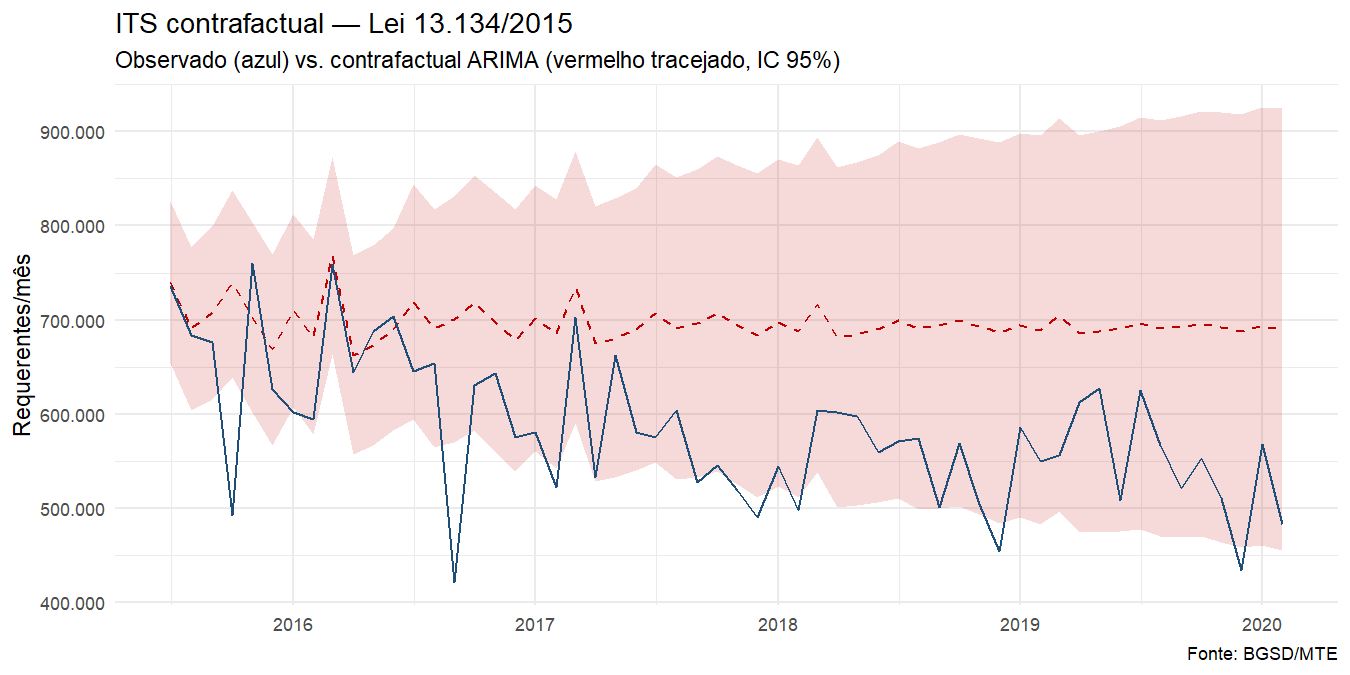
\includegraphics[width=\textwidth]{04_its_lei2015.png}
\caption{ARIMA-ITS: observado vs. contrafactual.}
\label{fig:its2015}
\end{subfigure}\hfill
\begin{subfigure}{0.49\textwidth}
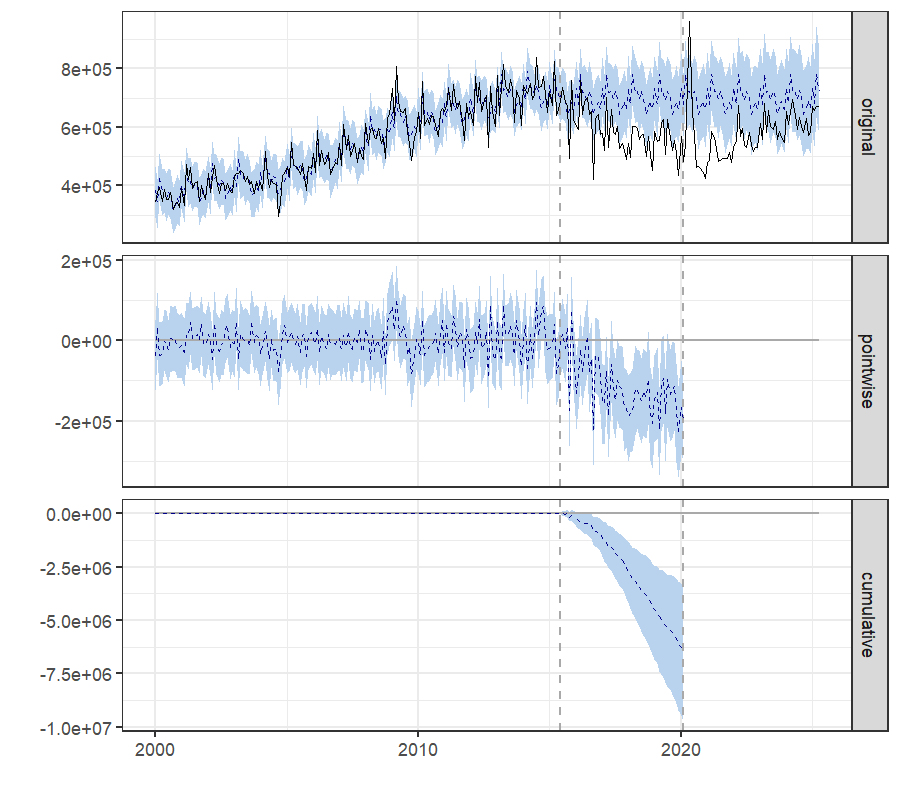
\includegraphics[width=\textwidth]{06_causalimpact_lei2015.png}
\caption{CausalImpact (sem controle).}
\label{fig:ci2015}
\end{subfigure}
\caption{Lei 13.134/2015: efeito estimado sobre os requerentes pelos dois métodos ITS, sem controle de demissões.}
\label{fig:lei2015}
\end{figure}

\subsection{Efeito condicional: o $-16\%$ desaparece ao controlar demissões}
O achado central está na Tabela~\ref{tab:controle}. Ao incluir as demissões do CAGED como controle no CausalImpact, o efeito estimado da Lei \textbf{muda de sinal e perde significância}: de $-16{,}4\%$ ($p\approx0{,}001$) para $+2{,}6\%$ ($p\approx0{,}15$), com o intervalo de credibilidade atravessando zero e \textbf{encolhendo pela metade} (de $\approx$\num{113495} para $\approx$\num{57520} de largura). Em outras palavras, uma vez que o contrafactual "sabe" o que aconteceu com as demissões, a queda de requerentes deixa de ser atribuível à reforma: ela é, em grande medida, a sombra da recessão de 2015--16 sobre o fluxo de separações (Figura~\ref{fig:cicontrole}).

\begin{table}[H]
\centering
\caption{CausalImpact da Lei 13.134/2015: sem vs. com controle de demissões (CAGED).}
\label{tab:controle}
\small
\begin{tabular}{lrrrr}
\toprule
Modelo & Efeito médio & Efeito \% & $p$-valor & Largura IC \\
\midrule
Sem controle            & $-$\num{115142} & $-16{,}4\%$ & 0,001 & \num{113495} \\
Com controle CAGED      & $+$\num{14267}  & $+2{,}6\%$  & 0,154 & \num{57520}  \\
\bottomrule
\end{tabular}
\\[4pt]
\footnotesize Fonte: elaboração própria. O controle reduz o efeito a zero estatístico e corta a incerteza pela metade.
\end{table}

\begin{figure}[H]
\centering
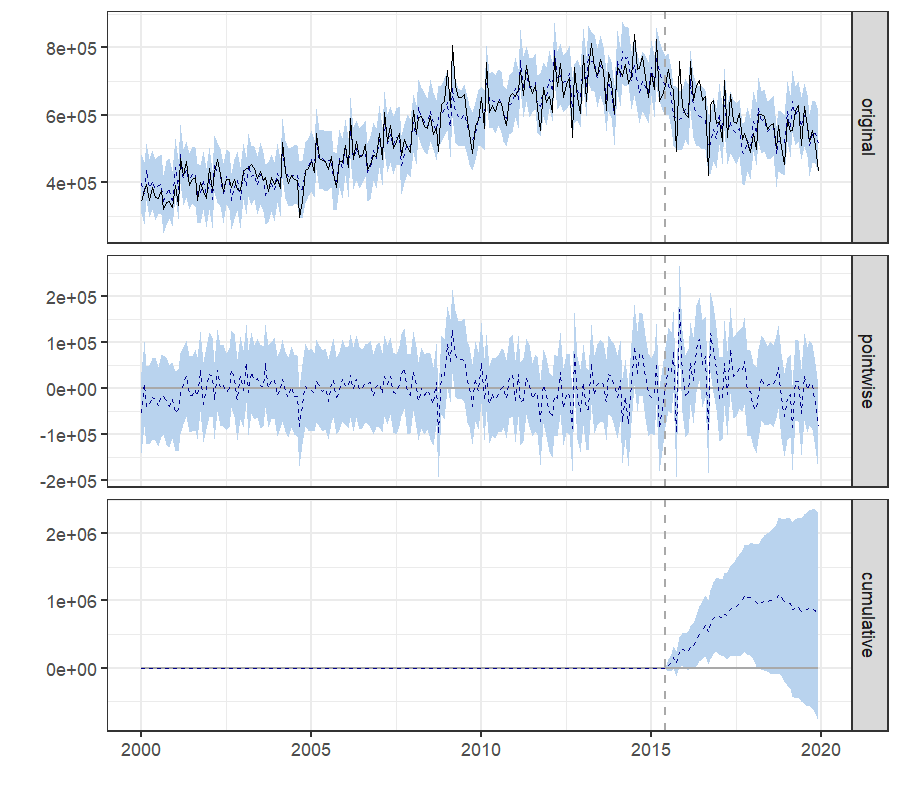
\includegraphics[width=0.85\textwidth]{09_causalimpact_lei2015_controle.png}
\caption{CausalImpact da Lei 13.134/2015 \textbf{com} controle das demissões do CAGED. O efeito pontual aproxima-se de zero e o intervalo de credibilidade cobre o nulo.}
\label{fig:cicontrole}
\end{figure}

\subsection{Taxa de habilitação: especificações divergem em sinal}
O teste da taxa de habilitação não resgata a identificação --- pelo contrário, expõe sua fragilidade. As quatro abordagens agregadas \textbf{divergem}, inclusive em sinal (Tabela~\ref{tab:taxa}): o nível sem controle dá $-16\%$; o condicional a demissões dá $\approx 0$; a taxa requerentes/demissões contra o contrafactual dá \textit{+10\%} ($p<0{,}01$); e a comparação de médias simples pré$\to$pós dá $-2\%$. A razão requerentes/demissões repica durante a recessão e depois reverte (Figura~\ref{fig:taxa}) --- um padrão \textbf{cíclico}, não um degrau de política. Como alertado, parte do "+10\%" é composição (mais dispensas involuntárias, elegíveis ao SD), não a Lei.

\begin{table}[H]
\centering
\caption{Quatro estimativas agregadas do efeito da Lei 2015 --- divergência de sinal.}
\label{tab:taxa}
\small
\begin{tabular}{lc}
\toprule
Abordagem & Efeito estimado da Lei 2015 \\
\midrule
Requerentes (nível), sem controle                 & $-16\%$ \\
Requerentes $\mid$ demissões (controle CAGED)      & $\approx 0$ (n.s.) \\
Taxa requerentes/demissões (vs. contrafactual)     & $+10\%$ ($p<0{,}01$) \\
Taxa requerentes/demissões (médias simples pré$\to$pós) & $-2\%$ \\
\bottomrule
\end{tabular}
\\[4pt]
\footnotesize Fonte: elaboração própria. Denominador = total de desligamentos (ressalva de composição no texto).
\end{table}

\begin{figure}[H]
\centering
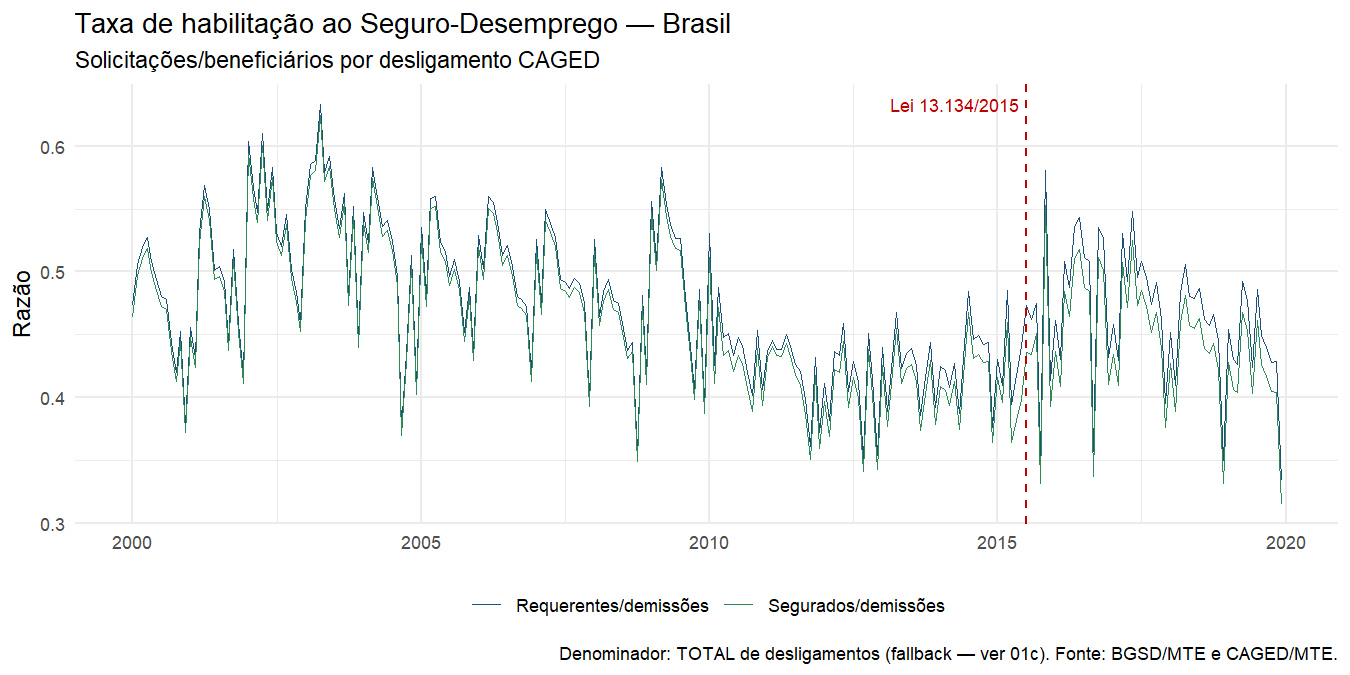
\includegraphics[width=0.85\textwidth]{10_taxa_habilitacao.png}
\caption{Taxa de habilitação (requerentes/demissões). O pico coincide com a recessão de 2015--16 e reverte em seguida --- dinâmica cíclica, não um degrau permanente de política.}
\label{fig:taxa}
\end{figure}

\subsection{COVID/2020: efeito líquido nulo}
Para completude, o choque pandêmico tem efeito líquido no primeiro ano estatisticamente indistinguível de zero em ambos os métodos ($+5{,}9\%$ no ARIMA-ITS, $+3{,}1\%$ no CausalImpact, $p\approx0{,}24$). Isso reflete a compensação entre o surto de demissões (abr--jun/2020) e a supressão posterior de desligamentos pela MP~936/BEm --- o pulso agudo é bem capturado pelo modelo com \textit{dummies} (coeficiente do pulso $\approx +$\num{301558}, altamente significativo), mas o efeito médio anual se cancela.

% =====================================================================
\section{Discussão: por que o agregado não identifica a Lei}
% =====================================================================

A convergência dos dois métodos em $-16\%$ é sedutora, mas enganosa. A reforma (jul/2015) coincidiu com a \textbf{maior recessão recente} do Brasil, que moveu \textit{simultaneamente} três coisas que se confundem no agregado: (i) o volume de demissões; (ii) a \textit{composição} das separações (mais dispensas involuntárias, elegíveis ao SD); e (iii) o \textit{take-up} do benefício. Cada especificação agregada carrega esse confundidor de uma forma diferente --- o que explica a divergência de sinal da Tabela~\ref{tab:taxa}. O teste decisivo (Tabela~\ref{tab:controle}) mostra que, uma vez condicionado o contrafactual na trajetória das demissões, a reforma não deixa pegada distinguível.

A leitura é consistente com \citet{schmiedervonwachter2016effects}, para quem efeitos de regras de SD estimados em janelas recessivas são particularmente difíceis de separar do ciclo. A implicação não é que a Lei não teve efeito, mas que \textbf{dados agregados nacionais não conseguem isolá-lo} da macroeconomia contemporânea.

\paragraph{O caminho para a identificação.} A solução reconhecida pela literatura brasileira \citep{brittopinottisampaio2022crime,gerardgonzaga2021informal} é explorar a \textbf{descontinuidade de elegibilidade} que a própria Lei criou. O desenho recomendado compara, em microdados ligados por PIS (RAIS/CAGED/BGSD), trabalhadores de primeira solicitação com vínculo logo abaixo do novo limiar (faixa $[6,12)$ meses --- que \textit{perdem} elegibilidade) contra trabalhadores com vínculo $\geq 12$ meses (sempre elegíveis), usando a terceira solicitação (regra inalterada) como placebo. Um grupo de controle que enfrenta a \textit{mesma} recessão faz o \textit{differencing-out} do confundidor macro --- precisamente o que o agregado não permite. Esse desenho (RD na elegibilidade e/ou diff-in-discontinuities, via \citealp{calonico2014robust,leelemieux2010rdd,callawaysantanna2021did}) permitiria, ademais, estimar desfechos de bem-estar (tempo até reemprego, salário no reemprego, transição para informalidade), e não apenas a contagem de solicitações.

% =====================================================================
\section{Conclusão}
% =====================================================================

Este artigo oferece a primeira avaliação quantitativa da reforma do seguro-desemprego de 2015 sobre o fluxo de requerentes, usando a série mensal completa (2000--2025) e a triangulação de dois métodos de série temporal interrompida. O resultado principal é uma \textbf{nota de não-identificação}: o efeito aparente de $-16\%$ em nível é um artefato da recessão de 2015--16 e não sobrevive ao controle pela dinâmica de demissões, com especificações concorrentes divergindo em sinal. O estudo delimita, assim, com rigor, o que os dados agregados conseguem sustentar e o que exige um desenho quase-experimental.

A contribuição é tanto substantiva --- documentar que a reforma de 2015 \textit{não} é identificável no agregado --- quanto metodológica: um estudo de caso de como a coincidência entre uma reforma e um choque macroeconômico corrói a identificação em ITS, e de como diagnosticá-la por triangulação e controle. O caminho à frente é o desenho de microdados na descontinuidade de elegibilidade $6\to12$ meses, apto a separar a Lei da recessão e a medir os desfechos de bem-estar que a literatura de desenho do SD considera centrais.

% =====================================================================
\bibliography{bib}
% =====================================================================

\end{document}
